%  !TeX  root  =  user_guide.tex

\section{Модуль OpenStreetMap}\label{plugins_osm}

% when the revision of a section has been finalized,
% comment out the following line:
% \updatedisclaimer

В последние годы проект OpenStreetMap стал очень популярен, потому что
во многих странах свободные геоданные, такие как например дорожная сеть
просто отсутствовали. Цель проекта OSM "--- создать свободноредактируемую
карту всего мира используя данные GPS, аэрофотосъемку или просто знание
местности. С тем, чтобы поддержать это начинание, QGIS предоставляет
плагин, который даёт пользователям возможность работать с данными OSM.

Плагин предоставляет всю базовую функциональность для работы с данными
OSM, загрузку данных, импорт, сохранение, скачивание, редактировани и
выгрузку обратно на сервер OpenStreetMap. Источником вдохновления при
создании плагина служили другие редакторы данных OSM. Цель авторов
плагина было объединение их функциональности и достижения наилучшего
результата.

Следующая секция дает краткое введение в принципы проекта OSM. Если вы
с ними уже знакомы, просто пропустите ее. Следующие параграфы были
частично позаимствованы с вебсайта OpenStreetMap по адресу
\url{http://www.openstreetmap.org}.

\minisec{Проект OpenStreetMap}

OpenStreetMap "--- проект который создаёт свободноредактируемую карту
мира. Карты создаются с помощью GPS, аэрофото и других источников, а
также знания местности. Проект появился потому что использование
большинства карт ограничено законодательно или технически, что
сдерживает их творческое использования способами которые раньше сложно
было представить. И изображения (тайлы) и векторные данные OSM доступны
для загрузки и имеют лицензию Creative Commons Attribution ShareAlike 2.0.

\begin{figure}[ht]
   \centering
   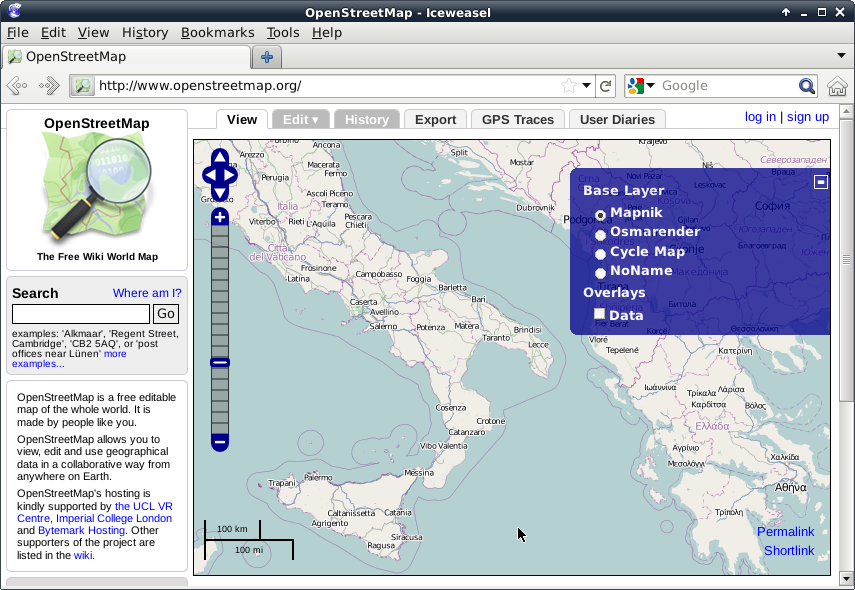
\includegraphics[clip=true, width=10cm]{osmweb}
   \caption{Данные OpenStreetMap в сети \nixcaption}\label{fig:osmweb}
\end{figure}

OpenStreetMap был вдохновлен такими проектами как Wikipedia "--- на карте
сайта (см. Рисунок~\ref{fig:osmweb}) есть большая закладка
\tab{Редактировать} и поддерживается полная история изменений.
Зарегистрированные пользователи могут загружать GPS треки и редактировать
векторные данные с помощью различных инструментов.

Структура данных OSM это класс объектов которые могут быть сохраненены с
помощью API на сервер. Три поддериваемых типа объектов это: \textbf{Узлы},
\textbf{Линии} и \textbf{Отношения}.

\begin{itemize}[label=--]
\item \textbf{Узел} это пара координат в системе широта/долгота. Он
используется для построения других объектов и как объект сам по себе
(например Точки интереса "--- POI) если он снабжен правильной атрибутикой.
\item \textbf{Линия} это список из минимум двух узлов, которые описывают
линейный объект такой как улица или что-то подобное. Узлы могут быть
участниками нескольких линий.
\item \textbf{Отношение} это группа из нуля или более примитивов с
назначенными ролями. Оно используется для указания отношений между
объектами, и может моделировать абстрактный объект.
\end{itemize}

Этими примитивами задаётся множество различных объектов карты
(<<Точка интереса>>, <<Улица>>, <<Трамвайная линия>>, <<Автобусная
остановка>> и т.\,п.). Атрибутика данных хорошо известна постоянным
участникам OSM и сохраняется в виде тегов, состоящих из ключа и
значения. Данные OSM обычно распространяются в формате XML. XML также
используется для обмена информацией с сервером OSM.

\minisec{Связь QGIS -- OSM}\label{qgis-osm-connection}

Первая часть этой секции описывает, как примитивы OSM показываются в
векторных слоях QGIS. Как было указано выше, данные OSM состоят из
Узлов, Линий и Отношений. В QGIS они показываются как три разных типа
слоёв: Точечный, Линейный и Полигональный. Убрать один из этих слоёв и
продолжить работу с другими "--- невозможно.

\begin{itemize}[label=--]
\item \textbf{Точечный слой} "--- показывает все объекты типа Узел,
которые являются самостоятельными. Это означает, что в этом слое будут
только Узлы которые не включены в Линии.
\item \textbf{Линейный слой} "--- показывает те объекты типа Линия
которые не замкнуты. Это означает, что ни одна из этих Линий не
начинается и заканчивается одинаковым Узлом.
\item \textbf{Полигональный слой} "--- показывает все Линии, не
включенные в Линейный слой.
\end{itemize}

Еще один примитив OpenStreetMap \textbf{Отношение}. Векторного слоя для
отображения специально нет. Отношение определяет взаимосвязи между любым
количеством объектов. После того, как Точка, Линия или Полигон отображены
на карте плагин показывает все отношения членом которых является примитив.

Связь между данными OSM и стандартными инструментами редактирования QGIS
было довольно сложно. Эти инструменты созданы для редактирования одного
векторного слоя единовременно, не важно какого типа объекты он показывает.
Это означает, что если данные OSM загружены в QGIS с помощью плагина, вы
теоретически должны мочь редактировать одновременно Точечный, Линейный и
Полигональный слои.

Проблема в том, что Линейный слой состоит из двух разных примитивов, Узлов
и Линий. Линии состоят из Узлов. Если вы начали редактировать Линейный
слой и изменили форму линейного объекта, ваши действия должны привести к
изменению не только Линий, но и Узлов, которые являются ее составляющими.

Стандартные инструменты редактирования QGIS не могут сказать провайдеру
OSM какие участники какой линии изменились и как. Они способны сказать
только какие новые участники появились, а этого недостаточно чтобы
правильно передать изменения в базу данных OSM. Линейный слой не знает
идентификаторов участников Линии. Те же самые проблемы возникают при
попытке редактирования слоя Полигонов.

Из этих соображений, плагину OSM нужны свои собственные инструменты
редактирования данных OSM. Когда для редактирования используются они,
изменение данных OSM осуществляется корректно. Инструменты редактирования
плагина включают средства создания, удаления и перемещения Точек, Линий,
Полигонов и Отношений.

\textbf{Примечание:} Для связи плагина OSM и стандартных инструментов
редактирования, необходимы изменения в ядре QGIS.

\subsection{Установка}

Плагин OpenStreetMap является плагином ядра QGIS. Если включена поддержка
Python плагин <<OpenStreetMap>> должен появиться в Менеджере плагинов и
он может быть выбран как описано в секции~\ref{sec:load_core_plugin}).

\subsection{Основной интерфейс пользователя}

При первом запуске плагина OSM и загрузки первых данных, появляются
несколько новых иконок на панели инструментов QGIS, а также несколько
новых графических компонент, показанных на Рисунке~\ref{fig:osmwidget}:

\begin{figure}[ht]
   \centering
   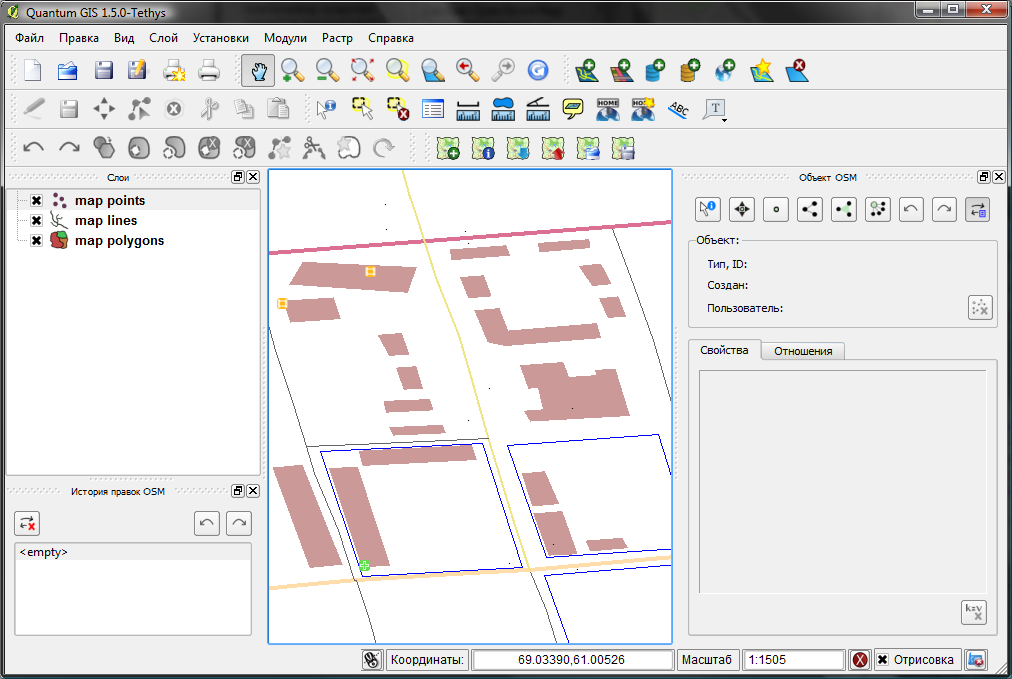
\includegraphics[clip=true, width=10cm]{osm_widgets}
   \caption{Интерфейс пользователя плагина OSM \nixcaption}\label{fig:osmwidget}
\end{figure}

\minisec{Панель объектов}

Панель объектов помогает идентифицировать объекты OSM. Она показывается
основную информацию о типе объекта и его идентификаторе, так же как
информацию о том кто и когда изменял этот объект. На панели объектов
также находятся все инструменты редактирования (в верхней части панели).
Инструменты редактирования более подробно освещены в секциях ниже.
Сначала панель заблокирована. Она разблокируется после успешной загрузки
некоторого количества данных OSM.

\minisec{Панель отмены/возврата}

Панель отмены/возврата используется для отмены и возврата действий
редактирования. На панели располагаются не только классические кнопки
отмены и возврата, но и список с кратким описанием предпринятых действий.
По умолчанию панель скрыта. Появляется панель после нажатия на
соответствующую кнопку на панели оъектов.

\minisec{Иконки основной панели инструментов}

\begin{description}
\item \toolbtntwo{osm_load}{Загрузить данные из файла} используется для
загрузки OSM из XML файла.
\item \toolbtntwo{osm_featureManager}{Показать/Скрыть панель объектов}
используется для открытия или скрытия панели объектов. Панель объектов
помогает просмотреть информацию об объекте, также на ней размещены
инструменты редактирования.
\item \toolbtntwo{osm_download}{Загрузить данные с сервера}
используется для загрузки данных с сервера OpenStreetMap.
\item \toolbtntwo{osm_upload}{Выгрузить данные} используется для
выгрузки изменений (относительно текущих данных).
\item \toolbtntwo{osm_import}{Импортировать данные из слоя}
используется для импорта данных из векторного слоя. Должен быть загружен
по крайней мере один векторный слой и должны быть выбраны данные OSM.
\item \toolbtntwo{osm_save}{Сохранить данные в файл} используется для
сохранения данных в файл XML.
\end{description}

Более детальная информация по каждой панели, кнопке и диалоге может быть
получена из соответствующих разделов этой документации, разделенной
согласно функциональности (редактирование, идентификация и т.д.).

\subsection{Загрузка данных OSM}

Первым делом после запуска плагина нужно открыть какие-то данные OSM.
Они могут быть загружены из файла или загружены непосредственно с
сервера. Здесь мы расскажем про первый метод.

Для загрузки данных из файла нажмите на кнопку
\toolbtntwo{osm_load}{Загрузить данные из файла} Если у вас нет такой
кнопки, возможно у вас отключен плагин, включите его заново выбрав
\mainmenuopt{Установки} \arrow \mainmenuopt{Панели} >
\dropmenuopt{OpenStreetMap}.

\begin{figure}[ht]
   \centering
   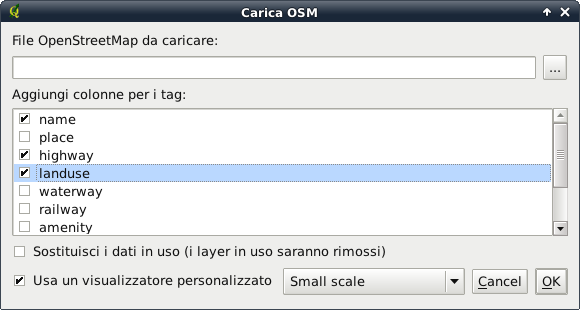
\includegraphics[clip=true, width=10cm]{osmloaddialog}
   \caption{Диалог загрузки данных OSM \nixcaption}\label{fig:osmload}
\end{figure}

Описание элементов диалога:

\begin{description}
\item \textbf{Загружаемый файл OpenStreetMap}: Нажмите на кнопку чтобы
выбрать файл .osm из которого нужны данные.
\item \textbf{Добавить колонки для тегов}: Эта опция определяет связь
между данными OSM и QGIS. Каждый объект OSM имеет теги (пары ключей и
значений), которые определяют свойства объекта. Каждый объект в QGIS
также имеет атрибуты (ключ и значение). Эта опция позволяет определить,
какие свойства объектов OSM должны быть видны, когда показывается
информация об объектах QGIS.
\item \textbf{Заменить текущие данные}: Включение этой опции означает,
что новые данные должны заменить существующие данные, с которыми
работает пользователь. Слои текущих данных будут удалены и загружены
новые. Когда данные загружаются в первый раз эта опция не активна, так
как заменять пока нечего.
\item \textbf{Использовать пользовательский рендерер}: Эта опция
определяет степерь детализации карты. Существует три уровня детализации
данных OSM. Используйте \button{Мелкий масштаб} если вам нужно
просматривать данные на уровне региона. Вы также можете использовать
\button{Средний масштаб} или \\
\button{Крупный масштаб}. Версия QGIS~\CURRENT не поддерживает
динамическую смену стиля рендеринга.
\end{description}

Нажмите \button{Ok} чтобы загрузить данные. Если это первая загрузка
файла, то сначала плагин должен обработать базу данных. Это может занять
несколько минут или секунд, в зависимости от количества данных.

\subsection{Просмотр данных OSM}

После того как данные OSM загружены, вы можете просмотреть информацию по
объектам используя инструмент \toolbtntwo{osm_identify}{Определить объекты}
расположенную справа в панели объектов OSM. Используя этот инструмент вы
можете легко изучить объекты на карте. Когда курсор мыши наведен на
объект, вы можете увидеть всю информацию о нем в панели объектов OSM.
Объект также подсвечивается на карте, так что пользователь может
определить что именно определилось.

Закладка \tab{Свойства} панели содержит все теги объекта. Включив
закладку \tab{Отношение} можно увидеть список всех отношений связанных
с текущим объектом.

Если вам нужно смотреть на параметры объекта и одновременное перемещать
курсор мыши, попробуйте щелкнуть левой кнопкой по объекту. Процесс
идентификации приостановится, пока вы не нажмете на левую кнопку мыши
снова.

Иногда в месте щелчка левой кнопкой находится более чем один объект.
Часто в такую ситуацию можно попасть при щелчке на перекресток или если
масштаб карты невелик. В этой ситуации определяется (и подсвечивается)
только один из объектов, но плагин запоминает их все. Потом, в режиме
паузы вы можете пролистать объекты по кругу правой кнопкой.

\subsection{Редактирование базовых данных}

Слово "базовых" в заголовке секции означает, что речь пойдет о всех
примитивах кроме отношений "--- узлах и линиях. Если вам нужна информация
о редактировании отношений, просто пропустите эту секцию и ознакомьтесь
со следующей.

Функции по редактированию базовых даных "--- основная часть плагина OSM.
Вы может изменять свойства, расположение или форму любого примитива. Вы
можете удалять объекты и добавлять новые. Все изменения узлов и линий
будут запомнены и их можно удобно отменить/вернуть и выгрузить на сервер
OpenStreetMap.

\minisec{Изменение тегов объектов}

Теги объектов можно изменять прямо в таблице тегов, которая
располагается в панели объектов. Не забудьте сначала выбрать объект.

\begin{figure}[ht]
   \centering
   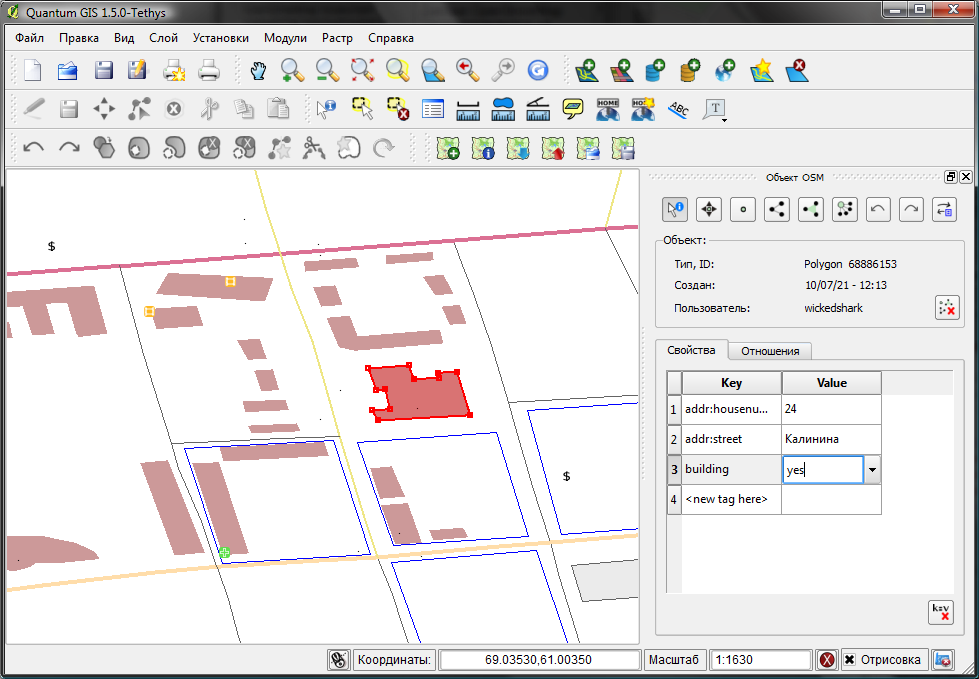
\includegraphics[clip=true, width=12cm]{osm_changefeaturetag}
   \caption{Изменение тега объекта OSM \nixcaption}\label{fig:osmchfeattag}
\end{figure}

Для изменения тега объекта, нужно дважды щелкнуть на соответствующей
строке колонки <<Значение>>, и ввести нужное значение. Если нужно удалить
тег, щелкните по ряду и используйте кнопку \button{Удалить выбранные теги}
находящуюся справа внизу таблицы.

Чтобы добавить новый тег, введите ключи и значение в последнюю строку
таблицы, где находится надпись '<следующее значение тега>'. Отметьте,
что вы не можете изменить ключ существующего тега. Для удобства ввода
тегов можно использовать подсказывающие комбо-списки уже заполненные
возможными ключами и их значениями.

\minisec{Создание точек}

Для создания точки служит кнопка \toolbtntwo{osm_createPoint}{Создать точку}
в панели объектов. Для создания точек, выберите этот инструмент и
щелкайте им по карте, созданные объекты сразу будут определяться. Если
вы щелкните по линии или полигону, будет создана точка на линии и
полигоне, как их часть. Если курсор находится над существующей точкой,
новая точка создана быть не может. В этом случае будет показано
следующее сообщение:

\begin{figure}[ht]
   \centering
   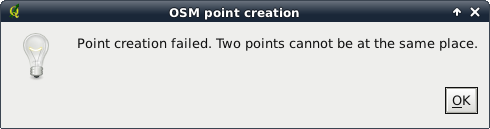
\includegraphics[clip=true, width=8cm]{osm_pointcreation}
   \caption{Сообщение при создании точки \nixcaption}\label{fig:osmpoicreat}
\end{figure}

Механизм помогающий пользователю точно попасть в линию или полигон
называется прищелкивание, он включен по умолчанию. Если нужно создать
точку очень близко к линии, но не на ней, нужно отключить прищелкивание
нажав клавишу \keystroke{Ctrl} перед нажатием.

\minisec{Создание линии}

Для создания линии служит инструмент \toolbtntwo{osm_createLine}{Создать линию},
кнопка которого располагается на панели объектов. Чтобы создать линию
выберите этот инструмент и начните щелкать левой кнопкой мыши на карте.
Каждый из щелчков превратится в узел "--- часть новой линии. Создание
линии завершается, когда вы первый раз щелкаете правой кнопкой мыши.
Линия сразу появится на карте.

\textbf{Note}: Линию с менее чем двумя узлами создать невозможно, в
случае если узел один, операция просто игнорируется.

Прищелкивание работает для всех узлов карты "--- точек из Точечного слоя
и всех узлов Линейного и Полигонального слоёв. Прищелкивание можно
отключить нажав \keystroke{Ctrl}.

\minisec{Создание полигона}

Создать полигон можно инструментом \toolbtntwo{osm_createPolygon}{Создать полигон},
кнопка которого располагается на панели объектов. Для создания полигона,
выберите инструмент и начните щелкать левой кнопкой на карте. Каждый из
щелчков превратится в узел "--- часть нового полигона. Создание полигона
будет завершено, когда вы первый раз щелкнете правой кнопкой мыши.
Полигон сразу появится на карте. Полигон из менее чем трех узлов создать
невозможно. В случае если узлов меньше трех, операция просто
игнорируется. Прищелкивание работает для всех узлов карты "--- точек из
Точечного слоя и всех узлов Линейного и Полигонального слоёв.
Прищелкивание можно отключить нажав \keystroke{Ctrl}.

\minisec{Перемещение объектов}

Если вы хотите передвинуть объект (не важно какого типа) используйте
инструмент \\
\toolbtntwo{osm_move}{Перемещение объектов} кнопка которого
располагается на панели объектов. Найдите объект, который нужно
переместить наведя на него курсор и щелкнув по нему. Если выберется не
тот объект не двигайте его, щелкните правой кнопкой пока не выберется
нужный. После того как объект выбран и вы переместили курсор,
прокручивать объекты больше будет нельзя. Для подтверждения перемещения,
щелкните левой кнопкой мыши, для отмены щелкните правой.

Если вы перемещаете объект связанный с другими объектами, эти связи не
будут нарушены. Другие объекты также могут видоизмениться чтобы
подстроиться к новому месту перемещенного объекта.

Для этой операции также поддерживается прищелкивание:

\begin{itemize}[label=--]
\item Когда перемещается отдельная точка, не являющаяся частью линии или
полигона, осуществляется прищелкивание ко всем сегментам и узлам.
\item Когда перемещается точка, являющаяся частью линии или полигона,
осуществляется прищелкивание ко всем сегментам и узлам, кроме узлов
родительских объектов.
\item Когда перемещается линия или полигон, осуществляется прищелкивание
ко всем узлам. Обратите внимание, что плагин пытается прищелкнуть только
к трём ближайшим к курсору узлам, иначе процесс был бы очень медленным.
Прищелкивание можно отключить удерживая \keystroke{Ctrl} в процессе.
\end{itemize}

\minisec{Удаление объектов}

Если нужно удалить объект, его сначала нужно идентифицировать. Далее,
чтобы его удалить, нужно использовать инструмент
\toolbtntwo{osm_removeFeat}{Удалить этот объект} кнопка которого
расположена на панели объектов. При удалении линии/полигона, удаляется
сама линия/полигон и все участвующие в ней узлы, которые не принадлежат
другой линии/полигону.

При удалении точки, которая является участником другой линии/полигона,
точка удаляется и изменяется геометрия родительской линии/полигона.
Новая геометрия имеет меньше узлов чем старая.

Если родительская геометрия является полигоном состоящим из трех узлов,
то у новой остается всего два. И так как, полигонов с двумя узлами быть
не может, тип объекта автоматически меняется на линию.

Если родительский объект был линией из двух точек, в новой геометрии
может остаться только одна. И так как линий из одного узла не бывает,
объект автоматически становится точкой.

\subsection{Редактирование отношений}\label{editing_osm_relation}

Благодаря существованию отношений, мы можем объединять объекты в группы
и назначать им общие свойства "--- таким образом мы можем смоделировать
любой возможный объект на карте: границы региона (как группу линий и
точек), маршрут автобуса и т.п. Каждый участник отношения имеет свою
особую роль. Этот плагин достаточно хорошо поддерживает работу с
отношениями и позволяет их изучать, создавать, обновлять и удалять.

\minisec{Изучение отношений}\label{examrelation}

Чтобы увидеть свойства отношения, нужно сначала определить одного из его
участников. После этого, откройте закладку \tab{Отношения} в панели
объектов. Ввеху закладки расположен список отношений частью которых
является выбранный объект. Выберите одно из них, которое нужно изучить,
снизу появится информация. В первой таблице <<Теги отношения>>
показываются свойства выбранного отношения. В таблице <<Участники
отношения>> можно найти информацию об участниках. Если нажать на одного
из них, плагин подсветит его на карте.

\minisec{Создание отношения}

Существует два пути создания отношения:

\begin{enumerate}
\item Можно использовать инструмент
\toolbtntwo{osm_createRelation}{Создать отношение} кнопка которого
находится на панели объектов.
\item Можно создать отношение в закладке \tab{Отношения} панели объектов
используя кнопку \\
\toolbtntwo{osm_addRelation}{Добавить отношение}.
\end{enumerate}

В обоих случаях появится новый диалог. Во втором случае, текущий объект
автоматически станет первым членом отношения. При создании отношения,
сначала укажите его тип. Можно выбрать один из предустановленных типов
или задать свой. После этого добавьте остальных участников отношения
и задайте теги.

Если тип отношения уже выбран, попробуйте использовать кнопку
\toolbtntwo{osm_generateTags}{Сгенерировать теги}. Она автоматически
создаст набор тегов, как правило соответствующих выбранному типу. Затем
нужно ввести соответствующие значения для ключей. Выбрать участников
отношения можно либо вводом их идентификаторов, типов и ролей или
использование инструмента \toolbtntwo{osm_identify}{Идентифицировать}
и указанием их на карте.

После того как тип, теги и участники отношения выбраны, можно дать
команду создать отношение.

\minisec{Изменение отношений}

Если нужно изменить существующее отношение, его необходимо сначала нужно
идентифицировать (как это объясняется в секции <<Изучение отношений>>).
После этого, нажмите на кнопку \\
\toolbtntwo{osm_editRelation}{Редактировать отношение}. Отношение
появится в панели объектов. Появится новый диалог, похожий на диалог
появляющийся при создании отношения. Окно будет заполнены значениями из
выбранного отношения. В нём можно изменять теги, участников и тип
отношения.

\subsection{Загрузка данных OSM}

Для загрузки данных с сервера OpenStreetMap нажмите на кнопку
\toolbtntwo{osm_download}{Загрузить данные}. Если кнопки не видно,
возможно не включена панель инструментов плагина. Её можно включить
обратно в \mainmenuopt{Настройки} \arrow \mainmenuopt{Панели} \arrow
\dropmenuopt{OpenStreetMap}.
После нажатия кнопки, появится диалоговое окно со следующими функциями:

\begin{figure}[ht]
   \centering
   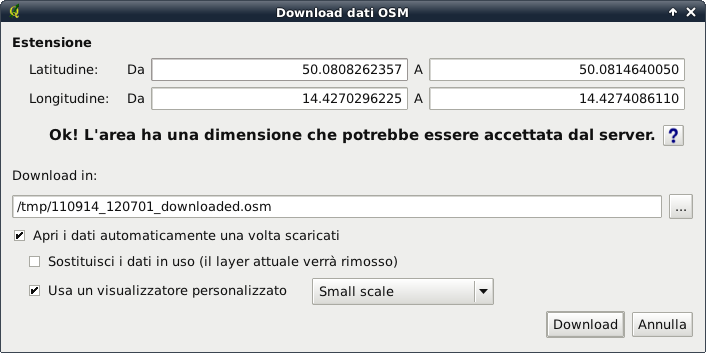
\includegraphics[clip=true, width=8cm]{osm_downloaddialog}
   \caption{Окно загрузки данных OSM \nixcaption}\label{fig:osmdownload}
\end{figure}

\begin{description}
\item \textbf{Охват}: Определяет географический охват загружаемых
данных в виде диапазонов широт и долгот. Поскольку существуют
определенные ограничения на максимальный объём загружаемых данных,
диапазоны координат не могут быть слишком широкими. Подробная информация
об ограничениях доступна по нажатию кнопки
\toolbtntwo{osm_questionMark}{Помощь} справа.
\item \textbf{Загрузить в}: Здесь указывается пусть к файлу, где будут
сохранены данные. Для указания другого пути можно использовать кнопку
\button{browse}.
\item \textbf{Открыть данные сразу после загрузки}: Определяет, если
после загрузки данные сразу должны быть открыты. Если загруженные данные
надо открыть позже, это можно сделать нажав кнопку \\
\toolbtntwo{osm_load}{Загрузить данные из файла}.
\item \textbf{Заменить текущие данные}: Эта опция активна только если
включено \\
\radiobuttonon{{}Открыть данные сразу после загрузки}. Включение этого
переключателя приведет к тому что загруженные данные заменят текущие.
Слои данных будут удалены и вместо них будут загружены новые. При первом
запуске QGIS и плагина эта опция будет неактивна, так как пока нечего
заменять.
\item \textbf{Использовать пользовательский рендерер}: Эта опция
активна только если включено \\
\radiobuttonon{{}Открыть данные сразу после загрузки}. Эта опция
определяет насколько детализированной будет карта. Существует три стиля.
Используйте \button{Мелкий масштаб} если вам нужно работать с данными
с низкой детализацией. Если нужно больше деталей, используйте
\button{Средний масштаб} или \button{Крупный масштаб}. QGIS~\CURRENT
не поддерживает динамическую смену стиля отрисовки.
\end{description}

Нажмите кнопку \button{Загрузить} чтобы начался процесс загрузки.

Индикатор прогресса будет показывать состояние процесса загрузки. Если
возникнет ошибка, появится окно объясняющее ее причину. После успешного
завершения индикатор прогресса и диалоговое окно закроются.

\subsection{Выгрузка данных}

Обратите внимание, что выгрузка всегда делается для текущего слоя. Перед
открытием диалога выгрузки убедитесь, что выбран правильный слой.

Для загрузки текущих данных на сервер OSM нажмите кнопку
\toolbtntwo{osm_upload}{Выгрузить данные}. Если кнопки не видно,
возможно не включена панель инструментов плагина. Её можно включить
обратно в \mainmenuopt{Настройки} \arrow \mainmenuopt{Панели} >
\dropmenuopt{OpenStreetMap}. После нажатия кнопки \button{upload}
появится диалоговое окно.

\begin{figure}[ht]
   \centering
   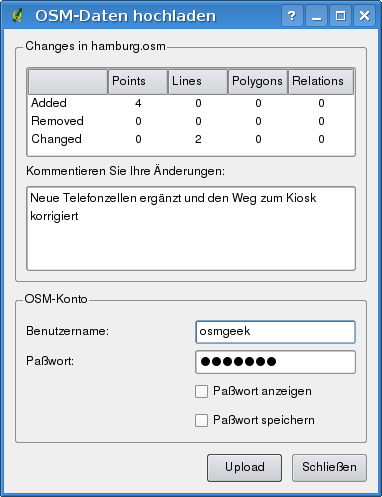
\includegraphics[clip=true, width=8cm]{osm_uploaddialog}
   \caption{Окно выгрузки данных OSM \nixcaption}\label{fig:osmupload}
\end{figure}

В верхней части окна можно проверить, те ли данные выгружаются по
указываемой там текущей базе данных. В таблице можно найти нформацию по
тому, сколько изменений будет выгружено. Статистика показывается
отдельно для каждого типа объектов.

В поле <<Комментарий для ваших изменений>> можно оставить краткое
описание изменений или не заполнять поле вообще. Заполните поля
<<Учётная запись OSM>>, чтобы сервер вас узнал. Если у вас нет учётной
записи в OSM "--- заведите ее по адресу \url{http://www.openstreetmap.org}.
После того, как все готово, нажмите \button{Выгрузить}, чтобы началась
выгрузка данных.

\subsection{Сохранение данных}

Чтобы сохранить данные текущего охвата карты в файл XML нажмите на кнопку
\toolbtntwo{osm_save}{Сохранить в файл}. Если кнопки не видно, возможно
не включена панель инструментов плагина. Её можно включить обратно в
\mainmenuopt{Настройки} \arrow \mainmenuopt{Панели} \arrow
\dropmenuopt{OpenStreetMap}. После нажатия кнопки появится диалоговое
окно.

\begin{figure}[ht]
   \centering
   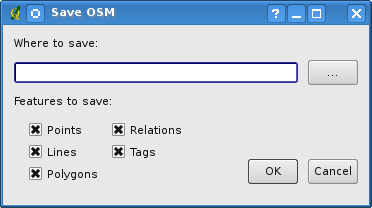
\includegraphics[clip=true, width=8cm]{osm_savedialog}
   \caption{Окно сохранения \nixcaption}\label{fig:osmsave}
\end{figure}

Выберите объекты, которые нужно сохранить в файл XML и его имя. Нажмите
\button{Ok} для начала процесса. Результатом будет файл XML содержащий
данные OSM с текущего охвата карты. Данные сохраняются в версии 0.6.
Некоторые элементы (<node>, <way>, <relation>) не содержат информации о
пакетах изменений и uid. Эта информация не является обязательной (см.
DTD для OSM XML версии 0.6). Выходные данные не сортируются.

Обратите внимание, что данные сохраняются в файл не строго по охвату.
Если в охват попадает только часть линии или полигона, они все равно
сохраняются целиком. Для каждой линии/полигона сохраняются все ее
участники.

\subsection{Импорт данных}

Чтобы импротировать данные из открытого векторного не-OSM слоя нужно:
Выбрать текущие данные OSM щелкнув на один из его слоёв. Выбрать
инструмент \toolbtntwo{osm_import}{Импортировать данные из слоя}. Если
такой кнопки нет, возможно не включена панель инструментов плагина. Её
можно включить обратно в \mainmenuopt{Настройки} \arrow \mainmenuopt{Панели}
> \dropmenuopt{OpenStreetMap}..

После нажатия появится следующее окно:

\begin{figure}[ht]
   \centering
   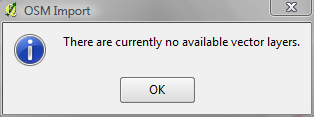
\includegraphics[clip=true, width=8cm]{osm_importdialog}
   \caption{Окно импорта данных \nixcaption}\label{fig:osmimportmessage}
\end{figure}

В этом случае не было загружено векторных слоёв. Загрузите один или
несколько слоёв, чтобы их можно было импортировать. Попробуйте нажать
кнопку еще раз (не забудьте отметить текущий слой данных OSM):

\begin{figure}[ht]
   \centering
   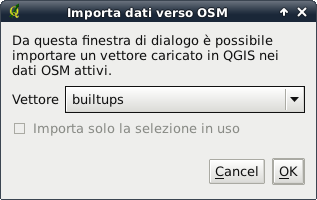
\includegraphics[clip=true, width=8cm]{osm_importtoosmdialog}
   \caption{Окно импорта данных \nixcaption}\label{fig:osmimporttoosm}
\end{figure}

Нажмите ОК чтобы начать процесс импорта.

\FloatBarrier
